%%%%%%%%%%%%%%%%%%%%%%%%%%%%%%%%%%%%%%%%%%%%%%%%%%%%%%%%%%%%%%%
%
% Welcome to Overleaf --- just edit your LaTeX on the left,
% and we'll compile it for you on the right. If you open the
% 'Share' menu, you can invite other users to edit at the same
% time. See www.overleaf.com/learn for more info. Enjoy!
%
%%%%%%%%%%%%%%%%%%%%%%%%%%%%%%%%%%%%%%%%%%%%%%%%%%%%%%%%%%%%%%%
\documentclass[aspectratio=169]{beamer}
\usepackage{graphicx}
\graphicspath{ {./Imagens/} }
\usepackage{graphicx}
\usetheme{PaloAlto}

%Information to be included in the title page:
\title{Cap.20 - Maximização do Lucro}
\author[Jean Haendell]{Jean Haendell Araújo Silveira}
\institute[UFC]{Universidade Federal do Ceará}
\date{7 de dezembro de 2022}

\begin{document}

\frame{\titlepage}

\begin{frame}
\frametitle{Introdução}
\begin{block}{Hipóteses Assumidas para a Construção do Modelo}
\begin{enumerate}
    \item A empresa encontra preços fixos para seus insumos e produtos;
    \item O mercado é \alert{competitivo}: isto é, um único produtor não consegue influenciar o preço;
    \item os mercados são competitivos tanto para os insumos quanto para os bens que a firma produz.
\end{enumerate}

    
\end{block}


\end{frame}

\begin{frame}{Lucros}

\begin{block}{ }

\begin{itemize}
    \item \alert{Lucros} são compostos de receitas menos custos.
    \item Suponhamos que a empresa produza n produtos $(y_1,...,y_n)$ e utilize m insumos $(x_1, ..., x_n)$. Sejam os preços dos bens produzidos $(p_1,...,p_n)$ e preço dos insumos $(w_1,...,w_n)$.

      O Lucro que a empresa recebe pode ser expresso como
    $$\pi = \sum_{i = 1}^{n} p_i y_i - \sum_{i = 1}^{m} w_i x_i $$
\end{itemize}


\end{block}
\end{frame}

\begin{frame}{Lucros}

\begin{block}{ }

\begin{itemize}
    \item Na expressão dos custos, devemos estar certo que incluímos \textit{todos} os fatores de produção utilizados pela empresa, a preços de mercado.
    \item Por exemplo, se a pessoa trabalha em sua própria empresa, o trabalho dela é um insumo e deve ser contado como parte dos custos.
    \item Ou seja, devemos levar em consideração os \alert{custos de oportunidade}.

\end{itemize}

\end{block}
\end{frame}

\begin{frame}{A Organização das Firmas}

\begin{block}{Tipos de empresas}

\begin{itemize}
    \item As empresas podem ser classificadas como:
    \begin{itemize}
    \item \alert{propriedade individual}: é uma empresa que é de propriedade de uma única pessoa.
    \item \alert{socidade}: é de propriedade de duas ou mais pessoas.
    \item \alert{sociedade anônima}: também é de propriedade de várias pessoas, mas perante a lei possui uma existência separada de seus donos.
    \end{itemize}

\end{itemize}


\end{block}
\end{frame}

\begin{frame}{Lucros e Valor no mercado de ações}

\begin{block}{ }

\begin{itemize}
    \item Imaginemos um mundo de certeza perfeita, onde o fluxo de lucros futuros da empresa seja de conhecimento público. Assim, o valor presente desses lucros seria o \alert{valor presente da empresa}, ou seja, quanto alguém estaria disposto a pagar para comprar a empresa.
    \item As participações de propriedade numa sociedade anônima são compradas e vendidas no \alert{mercado de ações}.
\end{itemize}

\end{block}
\end{frame}

%%%%% 

\begin{frame}{Lucros e Valor no mercado de ações}

\begin{block}{ }

\begin{itemize}
    \item O valor total de uma empresa no mercado de ações representa o valor presente do fluxo de lucros que a empresa deverá gerar.
    \item Portanto, em um mundo de certeza, o objetivo de maximizar o lucro pode ser entendido, também, como o objetivo de maximizar seu valor no mercado de ações.
\end{itemize}

\end{block}
\end{frame}

\begin{frame}{Lucros e Valor no mercado de ações}

\begin{block}{ }

\begin{itemize}
    \item Em um mundo de incerteza, maximizar o \textit{valor do mercado de ações} ainda possui significado.
    \item Portanto, maximizar o valor de mercado das ações gera uma função objetivo bem definida para empresas em quase todos os ambientes econômicos.
\end{itemize}

\end{block}
\end{frame}

\begin{frame}{Os Limites da Empresa}

\begin{block}{ }

\begin{itemize}
    \item Uma questão frequentemente enfrentada pelos gerentes de empresas é a de "fazer ou comprar".
    \item Há 40 anos, as próprias empresas proviam muito dos serviços. Hoje, tendem a terceirizar tanto quanto possível.
    \item Essa especialização costuma permitir que tais organizações ofereçam serviços de melhor qualidade e mais baratos às companhias que os utilizam.
\end{itemize}

\end{block}
\end{frame}

\begin{frame}{Fatores fixos e variáveis}

\begin{block}{ }

\begin{itemize}
    \item Referimo-nos a um fator de produção com uma quantidade fixa como um \alert{fator fixo}. Se o fator puder ser utilizado em quantidades diferentes, denominamo-lo de \alert{fator variável}.
    \item O curto prazo é definido como o período de tempo em que há alguns fatores fixos.
    \item No longo prazo, a empresa é livre para variar todos os fatores de produção.
\end{itemize}

\end{block}
\end{frame}


\begin{frame}{Maximização dos Lucros de Curto Prazo}

\begin{block}{ }

\begin{itemize}
    \item Seja $f(x_1,x_2)$ a função de produção da empresa, $p$ o preço do produto e sejam $w_1$ e $w_2$ os preços dos dois insumos. Então, o problema de maximização com o qual a empresa se depara pode ser escrito como $$\max_{x_1} pf(x_1,\bar{x_2}) - w_1 x_1 - w_2 \bar{x_2} $$
    
\end{itemize}

\end{block}
\end{frame}

\begin{frame}{Maximização dos Lucros de Curto Prazo}

\begin{block}{Condição para escolha ótima do fator 1}

\begin{itemize}
    \item Se $x^*_1$ for a escolha de maximização do lucro do fator 1, então $$pPM_1 (x_1^*, \bar{x_2}) = w_1$$ 
    \item Em outras palavras, \textit{o valor do produto marginal de um fator deve ser igual ao seu preço}.
\end{itemize}

\end{block}
\end{frame}

\begin{frame}{Maximização dos Lucros de Curto Prazo}

\begin{block}{ }

\begin{itemize}
    \item Ao utilizarmos y para representar a produção da empresa, os lucros são dados por $$\pi = py - w_1 x_1 - w_2 \bar{x_2}$$
    \item Essa expressão pode ser resolvida para y: $$ y = \frac{\pi}{p} + \frac{w_2}{p} \bar{x_2} + \frac{w_1}{p} x_1$$
\end{itemize}

\end{block}
\end{frame}


\begin{frame}{Maximização dos Lucros de Curto Prazo}

\begin{block}{ }

\begin{itemize}
    \item Essa equação descreve as retas isolucro, que são combinações de insumos e de produtos que fornecem um nível constante de lucros, $\pi$. 

    
     \centering 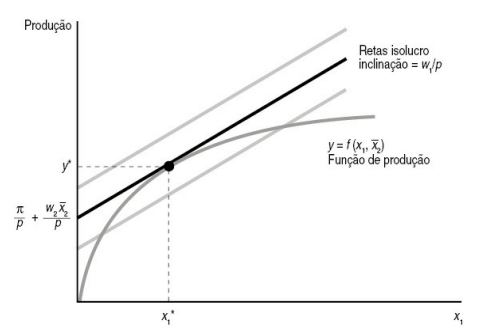
\includegraphics[scale = 0.5]{grafico1}
    
  
\end{itemize}

\end{block}
\end{frame}

\begin{frame}{Estática Comparativa}

\begin{block}{ }

\begin{itemize}
    \item Quando o preço do fator 1 aumenta, a demanda pelo fator 1 tem de diminuir.
    \item Em termos de Cálculo, nós queremos examinar a derivada parcial de $x^*_1$ em relação a $w_1$. $$ \frac{\partial x_1^*}{\partial w_1} = \frac{1}{p \frac{\partial^2 f(x_1^* , \bar{x_2})}{\partial^2 x_1^*}} < 0$$
    
    
  
\end{itemize}

\end{block}
\end{frame}

\begin{frame}{Maximização do Lucro no Longo Prazo}

\begin{block}{ }

\begin{itemize}
    \item No longo prazo, a empresa é livre para escolher o nível de todos os insumos. Então, o problema de maximização no longo prazo pode ser descrito como $$\max_{x_1} pf(x_1, x_2) - w_1 x_1 - w_2 x_2  $$
    \item Portanto, as condiçoes de primeira-ordem implicam $$pMP_1 (x^*_1, x^*_2) = w_1$$ e

    $$pMP_2 (x^*_1, x^*_2) = w_2$$
    
    
  
\end{itemize}

\end{block}
\end{frame}

\begin{frame}{Maximização do Lucro no Longo Prazo}

\begin{block}{ }

\begin{itemize}
    \item As equações resultantes são chamadas de \alert{curvas de demanda de fatores.}
    
  
\end{itemize}

\end{block}
\end{frame}

\begin{frame}{Curvas de demanda inversas de fatores}

\begin{block}{ }

\begin{itemize}
    \item As \alert{curvas de demanda de fatores} de uma empresa medem a relação entre o preço de um fator e a escolha maximizadora do lucro daquele fator.
    \item A \alert{curva de demanda inversa de fatores} mede quais devem ser os preços dos fatores para que se demande determinada quantidade de insumos.
\end{itemize}

\end{block}
\end{frame}

\begin{frame}{Lucratividade revelada}

\begin{block}{ }

\begin{itemize}
    \item Vamos supor que observamos duas escolhas que a empresa faz em dois conjuntos
diferentes de preços. No período $t$, ela se depara com os preços $(p^t , w^t_1, w^t_2)$ e faz as escolhas $(y^t, w^t_1 , x^t_2)$. No período $s$, depara-se com os preços $(p^s , w^s_1, w^s_2)$ e faz as escolhas $(y^s, w^s_1 , x^s_2)$. 
\end{itemize}

\end{block}
\end{frame}

\begin{frame}{Lucratividade revelada}

\begin{block}{ }

\begin{itemize}
    \item Se a função de produção da empresa não mudar entre os períodos s e t e se a empresa for maximizadora de lucro, deveremos ter $$p^t y^t - w^t_1 x^t_1 - w^t_2 x^t_2 \geq p^t y^s - w^t_1 x^s_1 - w^t_2 x^s_2$$

    \centering e
$$p^s y^s - w^s_1 x^s_1 - w^s_2 x^s_2 \geq p^s y^t - w^s_1 x^t_1 - w^s_2 x^t_2$$
    
\end{itemize}

\end{block}
\end{frame}

\begin{frame}{Lucratividade revelada}

\begin{block}{ }

\begin{itemize}
    \item Se qualquer uma dessas desigualdades fosse violada, a empresa não poderia ter sido maximizadora do lucro.
    \item A satisfação dessas duas desigualdades constitui virtualmente um axioma do comportamento maximizador do lucro, podendo, pois, receber o nome de \alert{Axioma Fraco de Maximização do Lucro (AFML)}.
\end{itemize}

\end{block}
\end{frame}

\begin{frame}{Lucratividade revelada}

\begin{block}{ }

\begin{itemize}
    \item À medida que observamos um número maior de escolhas, obtemos uma estimativa mais precisa da função de produção.
    \item Essa estimativa da função de produção pode ser utilizada para prever o comportamento da empresa em outros ambientes ou para outros usos em análise econômica.
    
\end{itemize}

\end{block}
\end{frame}

\begin{frame}{Minimização do Custo}

\begin{block}{ }

\begin{itemize}
    \item Se uma empresa maximiza os lucros e escolhe ofertar uma quantidade de produtos y, então ela tem de minimizar o custo de produzir y. Se não fosse assim, existiria um meio mais barato de produzir y unidades do produto, o que significaria que a empresa, em primeiro lugar, não estaria maximizando lucros.
\end{itemize}

\end{block}
\end{frame}

\begin{frame}{Referências Bibliográficas}

\begin{block}{ }

\begin{itemize}
    \item VARIAN, Hal R. Intermediate Microeconomics with Calculus : a Modern Approach. New York :W.W. Norton & Co., 2014.
    \item VARIAN, Hal R. Microeconomia: uma abordagem moderna. 8.ed. Rio de Janeiro: Elsevier, 2012
\end{itemize}

\end{block}
\end{frame}

\end{document}




